\documentclass[./main.tex]{subfiles} 
\begin{document}

\subsection{Time-Frequency Estimation}

\subsubsection{Experimenting with the Spectrogram}

\subsubsection{Spectrogram of Real-World EEG Data}

\begin{figure}[h]
	\centering 
	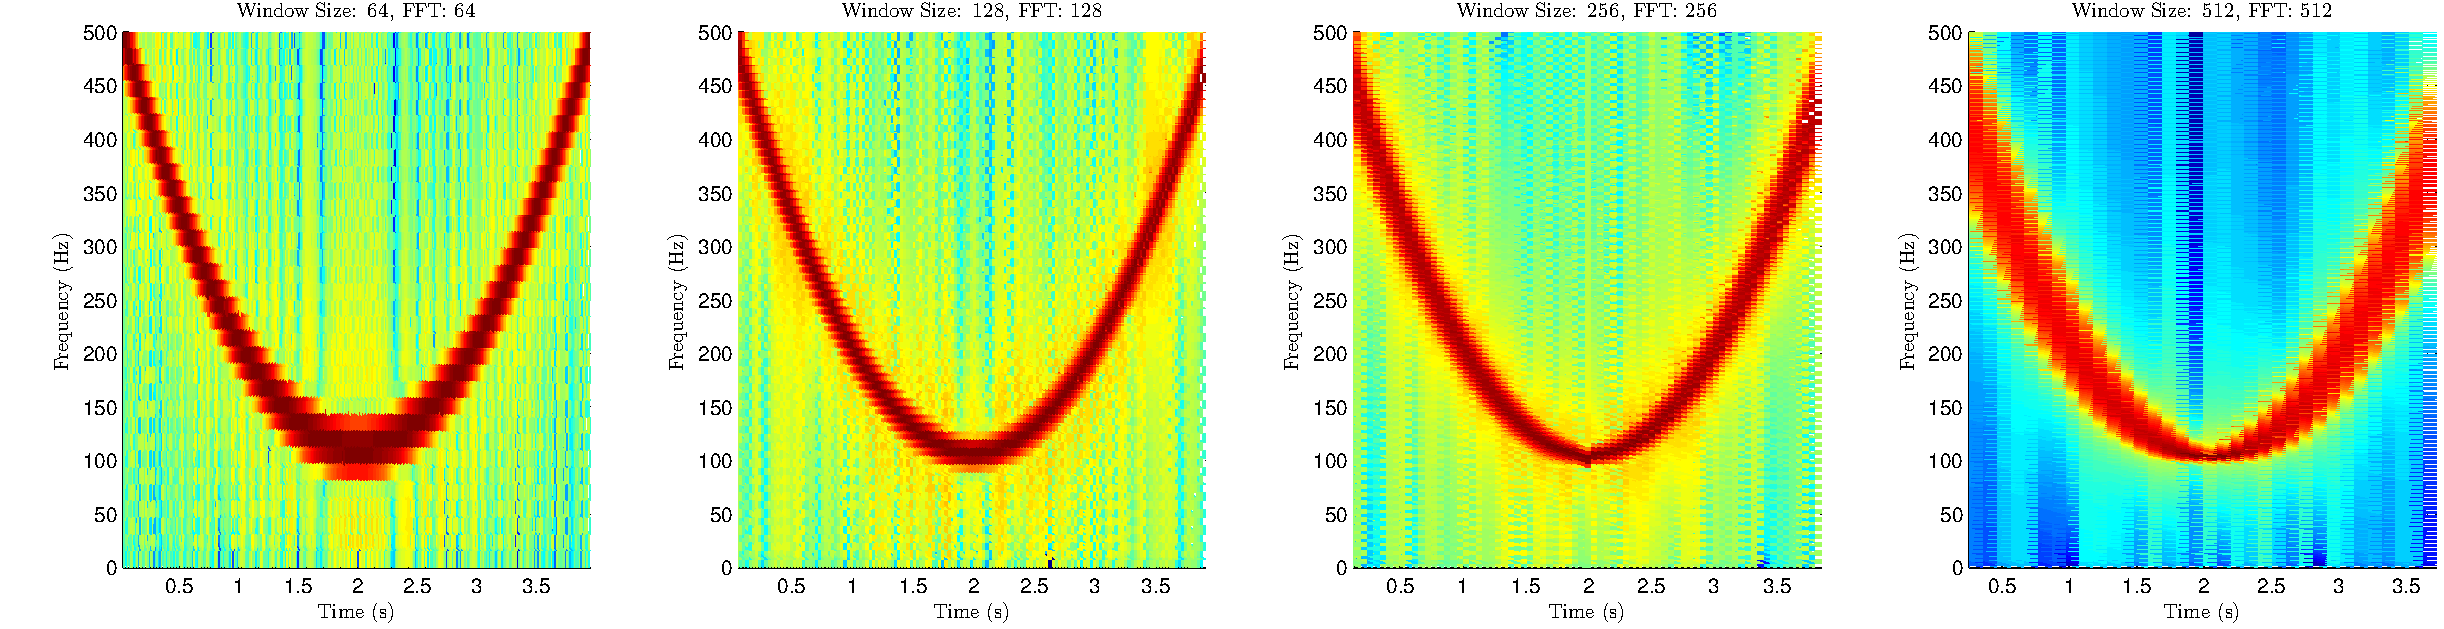
\includegraphics[scale=0.45]{fig/2/2_3_a_window_size.pdf}
	\caption{\textit{Circularity Plots for Wind Data}}
	\label{fig:}
\end{figure}

\begin{figure}[h]
	\centering 
	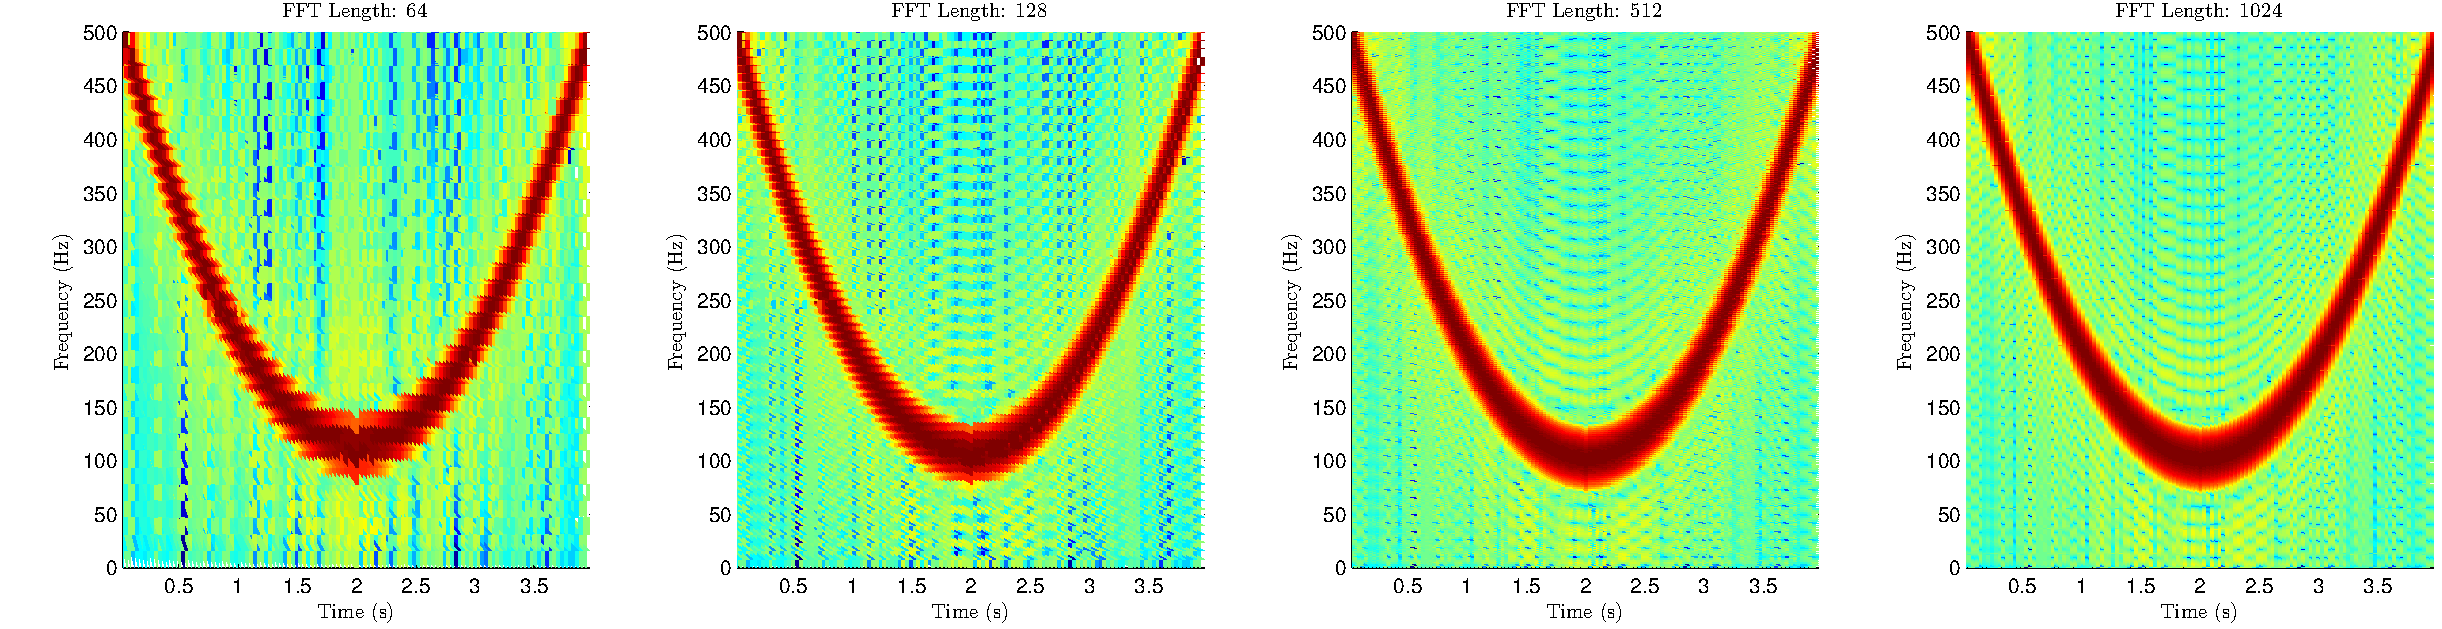
\includegraphics[scale=0.45]{fig/2/2_3_a_fft_len.pdf}
	\caption{\textit{Circularity Plots for Wind Data}}
	\label{fig:}
\end{figure}

\begin{figure}[h]
	\centering 
	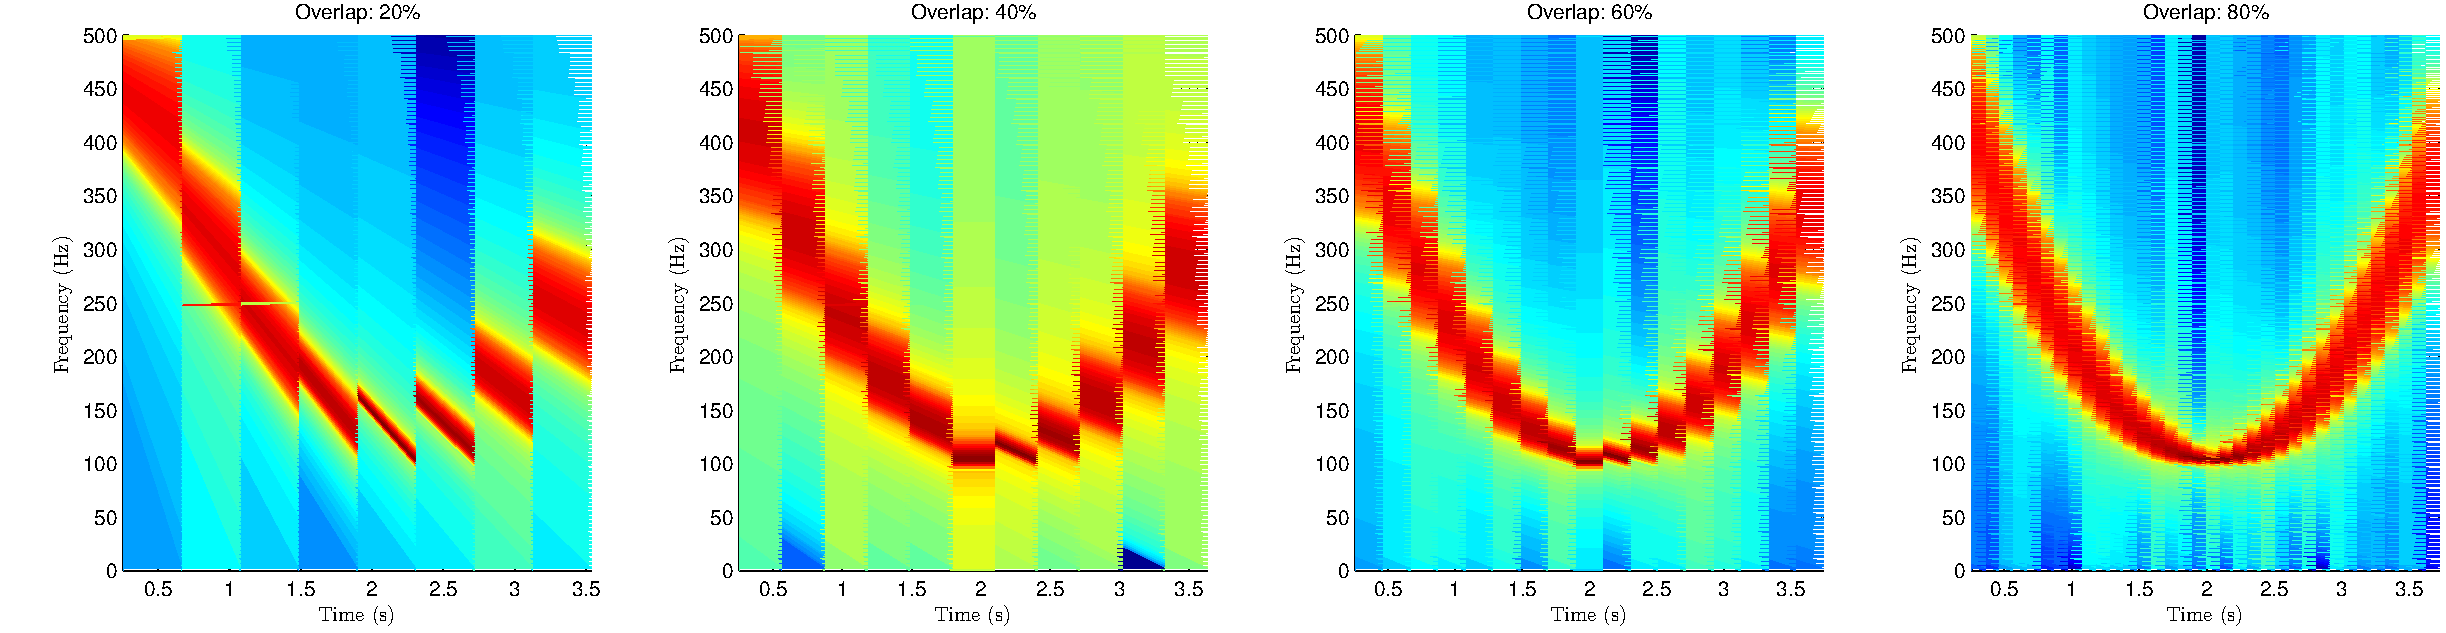
\includegraphics[scale=0.45]{fig/2/2_3_a_overlap.pdf}
	\caption{\textit{Circularity Plots for Wind Data}}
	\label{fig:}
\end{figure}

\begin{figure}[h]
	\centering 
	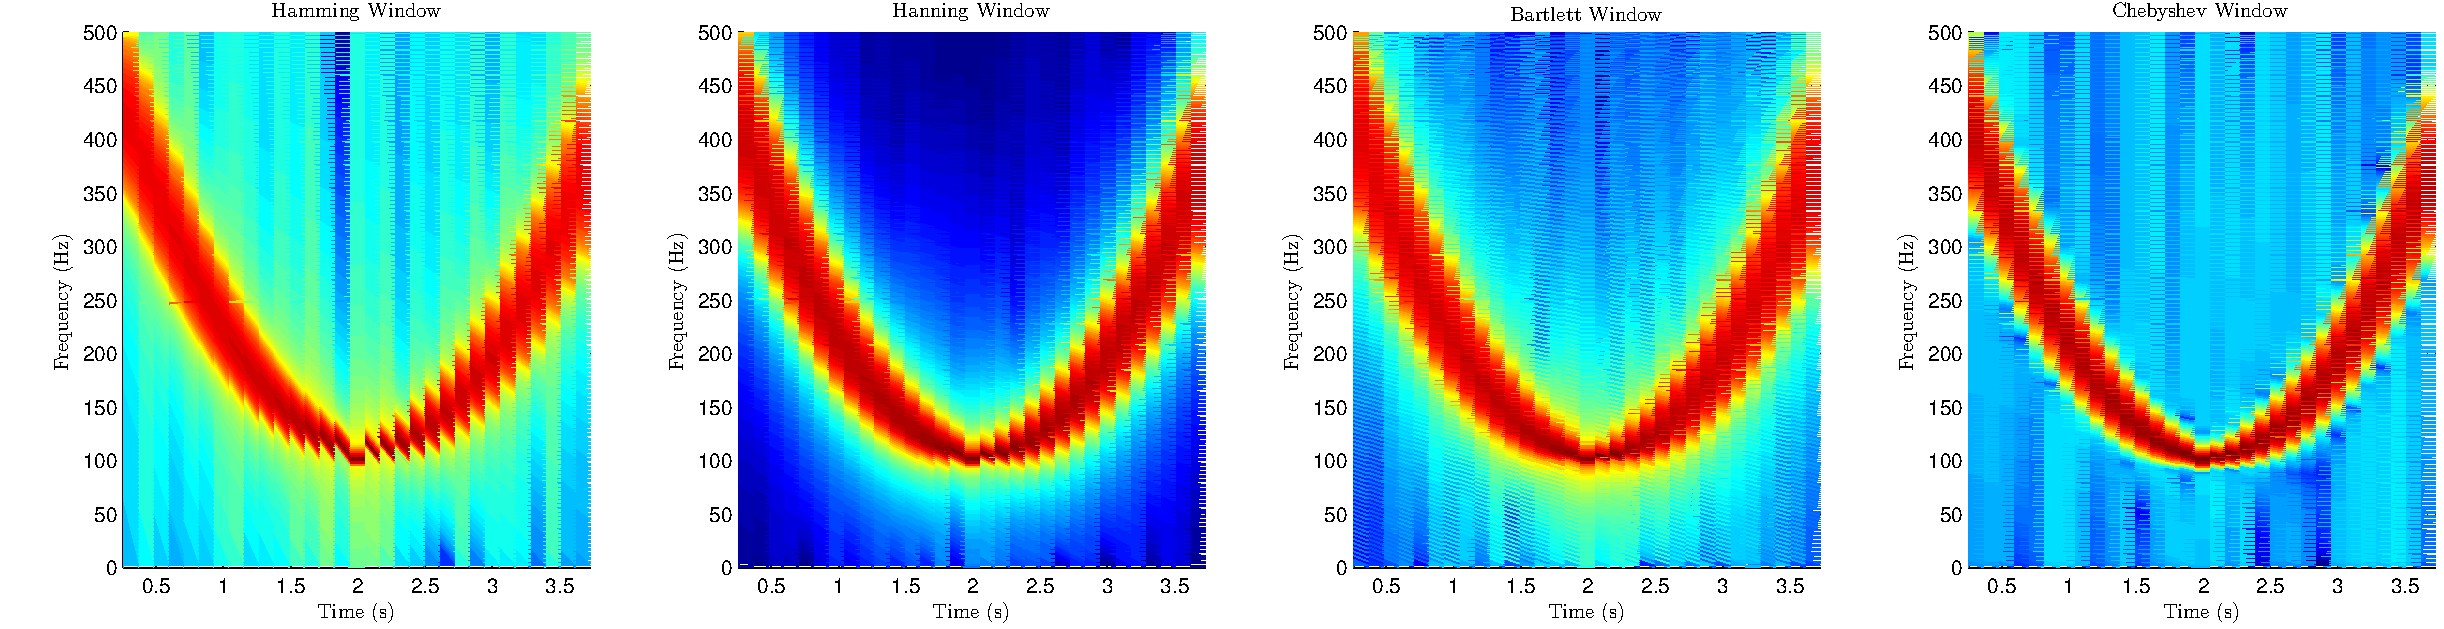
\includegraphics[scale=0.45]{fig/2/2_3_a_windows.pdf}
	\caption{\textit{Circularity Plots for Wind Data}}
	\label{fig:}
\end{figure}
%\begin{figure}[h]
%	\centering 
%	\resizebox{\textwidth}{!}{\input{fig/2/2_3_a_overlap.tikz}}
%	\caption{\textit{Circularity Plots for Wind Data}}
%	\label{fig:2_2_b}
%\end{figure}
%
%\begin{figure}[h]
%	\centering 
%	\resizebox{\textwidth}{!}{\input{fig/2/2_3_a_fft_len.tikz}}
%	\caption{\textit{Circularity Plots for Wind Data}}
%	\label{fig:2_2_b}
%\end{figure}
%
%\begin{figure}[h]
%	\centering 
%	\resizebox{\textwidth}{!}{\input{fig/2/2_3_a_window_types.tikz}}
%	\caption{\textit{Circularity Plots for Wind Data}}
%	\label{fig:2_2_b}
%\end{figure}

\end{document}

